\chapter{Визуализация моделей конструктивной блочной геометрии} \label{chapt2}

Конструктивная блочная геометрия (Constructive Solid Geometry или CSG) \cite{Requicha80} представляет собой подход к геометрическому моделированию твердых, который сводится к составлению сложных тел из более простых геометрических примитивов. В отличие от подходов поверхностного моделирования, CSG используется для твердотельного моделирования, так как CSG модель задает и поверхность и объем тела.

Настоящая глава определяет модели конструктивной геометрии в терминах \textit{примитивов}, \textit{операций} и \textit{деревьев}. Описаны обход и обработка CSG деревьев. В контексте CSG визуализации, трансформация и симплификация дерева производятся как предварительные шаги, необходимые для последующей эффективной визуализации.

Настоящая глава приводит основные модели и алгоритмы используемые для CSG визуализации.

\todo{дописать}

\section{Примитивы} \label{sect_primitives}

Геометрические объекты используемые в CSG моделировании называют \textit{примитивами}. Примитивы определяют свой объем, разделяя пространство на внутреннюю и внешнюю области. Поверхность примитива находится на границе между внутренней и внешней областями.

Набор примитивов доступных в системах CSG моделирования обычно состоит из сфер, эллипсоидов, параллелепипедов, тетраэдров, цилиндров, конусов и торов. Как правило, все примитивы параметризованы. Формально, набор примитивов определяет только типы поверхности, доступные для CSG моделирования, однако на практике, для удобства пользователя, могут использоваться избыточные и составные примитивы (переиспользуемые CSG поддеревья). \todo{картинка с примитивами} Некоторые системы также поддерживают триангулированные объекты при условии что те однозначно определяют внутреннюю и внешнюю область примитива.

\todo{ограниченный vs замкнутый}

Примитивы могут быть ограниченными и неограниченными и, соответственно, занимать конечный или бесконечный объем. Неограниченные примитивы, такие как плоскости, параболоиды, неограниченные цилиндрические и конические поверхности, могут использоваться в CSG моделировании. Однако при использовании неограниченных примитивов нельзя гарантировать что результат CSG выражения представляет собой твердое тело конечного объема.

Компьютерная графика часто имеет дело, главным образом, с поверхностями объектов, так как они и формируют в конечном счете видимое изображение. Однако, в CSG моделировании и визуализации, объем тела имеет не меньшее значение.

\section{Операции} \label{sect_operations}

\todo{множества}

CSG примитивы могут быть скомбинированны в более сложные объекты при помощи операций \todo{булевой алгебры}. Основные операции включают в себя \textit{объединение}, \textit{пересечение} и \textit{разность}. Настоящая работа использует нотацию операций над множествами $\cup$, $\cap$ и $\setminus$ для объединения, пересечения и разности соответственно.

\noindent Для примитивов $a$ и $b$:
\begin{itemize}
  \item \textit{Объединение} обозначается как $a \cup b$ и представляет собой совокупный объем занимаемый примитивами $a$ и $b$, а также поверхность $a$ не содержащуюся внутри $b$ и поверхность $b$ не содержащуюся внутри $a$.

  \item \textit{Пересечение} обозначается как $a \cap b$ и представляет собой объем занимаемый одновременно примитивами $a$ и $b$, а также поверхность $a$ содержащуюся внутри $b$ и поверхность $b$ содержащуюся внутри $a$.

  \item \textit{Разность} обозначается как $a \setminus b$ и представляет собой объем занимаемый примитивом $a$ и при этом находящийся вне примитива $b$, а также поверхность $a$ не содержащуюся внутри $b$ и поверхность $b$ содержащуюся внутри $a$.
\end{itemize}

Объединение, пересечение и разность показаны на Рисунке~\ref{fig:operations} (а), (б) и (в) соответственно.

\begin{figure}[ht]
  \begin{minipage}[ht]{0.3\linewidth}\centering
    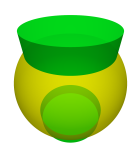
\includegraphics[width=0.6\linewidth]{union} \\ а)
  \end{minipage}
  \hfill
  \begin{minipage}[ht]{0.3\linewidth}\centering
    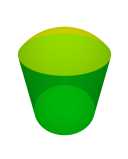
\includegraphics[width=0.6\linewidth]{intersection} \\ б)
  \end{minipage}
  \hfill
  \begin{minipage}[ht]{0.3\linewidth}\centering
    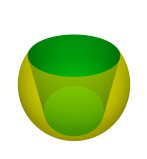
\includegraphics[width=0.6\linewidth]{difference} \\ в)
  \end{minipage}
  \caption{CSG операции}
  \label{fig:operations}  
\end{figure}

\section{CSG дерево} \label{sect_csg_tree}

CSG дерево это иерархическая модель в которой листовые узлы соответствуют базовым примитивам, а внутренние узлы "--- булевым операциям. Дочерним узлом внутреннего узла может быть примитив либо операция. Примитивы, в свою очередь, не имеют дочерних узлов. Корень дерева (узел не имеющий родительских узлов) соответствует объекту, который моделируется CSG деревом. Рисунок~\ref{fig:example_tree} изображает CSG модель, состоящую из сферы, параллелепипеда и двух цилиндров: $(((a \cap b) \setminus c) \setminus d)$. В этом примере узлы $a$, $b$, $c$ и $d$ являются примитивами (листовыми узлами), а остальные внутренними узлами.

Иерархические геометрические модели и CSG дерево, в частности, как правило, позволяют задать матрицу трансформации для любого из узлов. Таким образом, возможно задавать перенос, поворот и масштаб для отдельных примитивов и целых поддеревьев. По соглашению, трансформация применяется отностительно родительского узла и задает локальную систему координат для каждого узла дерева. Наличие локальной системы координат часто требуется для удобства интерактивного редактирования дерева и анимации.

CSG деревья обычно представляют как двоичные деревья "--- каждая операция имеет ровно два дочерних узла. Для сокращения записи можно использовать узлы произвольной арности ($\ge 2$), однако такое дерево всегда можно свести к бинарному.

\begin{figure} 
  \centering
  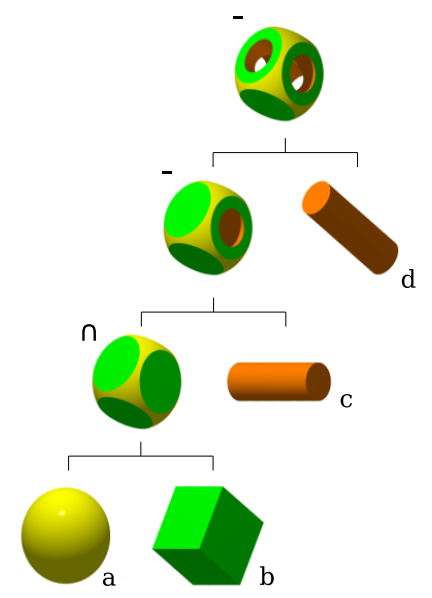
\includegraphics [scale=0.5] {example_tree}
  \caption{Пример CSG дерева}
  \label{fig:example_tree}
\end{figure}

\section{Обход} \label{sect_csg_traversal}

Алгоритмы на CSG деревьях, как правило, основаны на процедуре \textit{обхода} (англ. traversal) дерева "--- посещения каждого внутреннего и листового узла дерева в точности один раз. Обход начинается с корня дерева и доходит до листовых узлов рекурсивно. Такие обходы классифицируются по порядку, в котором узлы посещаются:

\begin{itemize}
  \item \textit{Прямой обход} (англ. pre-order traversal) посещает узел перед рекурсивным обходом левого и затем правого поддеревьев.

  \item \textit{Центрированный обход} (англ. in-order traversal) рекурсивно обходит левое поддерево, посещает текущий узел и далее правое поддерево.

  \item \textit{Обратный обход} (англ. post-order traversal) рекурсивно обходит левое и правое поддерево и затем посещает узел.
\end{itemize}

Центрированный обход можно использовать для получения CSG выражения для заданного дерева, слева направо. Например для CSG дерева на Рисунке~\ref{fig:example_tree} выражение будет выглядеть так: $(((a \cap b) \setminus c) \setminus d)$.

\section{Алгоритмы} \label{sect_csg_algo}

Настоящая работа сфокусирована на проблеме интерактивной визуализации конструктивных моделей, однако CSG подход позволяет эффективно решать ряд других задач геометрического моделирования. В данном разделе приводятся некоторые общие алгоритмы на CSG деревьях.

Задача \textit{классификации точки} (англ. point classification) состоит в том, чтобы определить в какой области пространства лежит заданная точка, внутри или снаружи CSG модели. Начиная с корня, рекурсивный обратный обход сначала классифицирует точку относительно дочерних узлов. Результат в каждом внутреннем узле определяется путем применения булевых операций к дочерним классификациям. Таким образом, классификация точки может быть реализована для сложных объектов, основываясь лишь на простых операциях классификации точки относительно примитивов.

Задача \textit{классификации линии} (англ. line classification) состоит в том, чтобы разделить линию на сегменты находящиеся внутри и снаружи CSG модели, а также точки находящиеся на поверхности модели. Классификация линии может быть выполнена схожим образом с классификацией точки, путем классификации линии относительно примитивов и применению булевой логики к дочерним интервалам на линии.

Задача \textit{бросания луча} (англ. ray casting) определяет первую точку пересечения заданного луча с поверхностью конструктивной модели. Эту задачу можно решить путем классификации линии и поиска ближайшей поверхности к началу луча в направлении луча. Однако, задача бросания луча является более частной чем задача классификация линии и может быть выполнена эффективнее. Эффективная реализация алгоритма бросания луча для CSG модели описана в Главе \ref{chapt3} и лежит в основе решения, описанного в настоящей работе.

Задача \textit{определения видимости} (англ. visibility query) может быть реализована с помощью бросания лучей.

Задача \textit{обнаружения столкновений} (англ. collision detection) требует определения области контакта, либо пересечения нескольких объектов. Пересечение CSG моделей может быть выражено как операция пересечения примененная к паре CSG моделей. Дальнейший анализ необходим для определения существования, а также конкретного вида области пересечения.

Задача \textit{выделения границы} (англ. boundary evaluation) сводится к переводу модели в граничное представление. В таком представлении поверхность модели задана явно в виде вершин, ребер и граней. Такое представление используется для расчета площади поверхности и прочих задач анализа поверхности, произведения геометрических операций, а также визуализации. Применимость операции выделения границы для задач интерактивной визуализации ограничивает трудоемкость этой операции для сложных моделей.

CSG модель также может быть представлена в воксельном представлении с заданной точностью. В этом представлении такие задачи как вычисление объема тела, классификация точки и бросания луча выполняются эффективнее. Однако, как и в случае с выделением границы, переход к воксельному представлению это ресурсоемкий процесс.

\section{Трансформация CSG дерева} \label{sect_csg_transform}

Узлы CSG дерева могут быть перемещены при сохранении того же объема и поверхности результирующей модели. Трансформация CSG дерева часто является необходимым предварительным шагом для последующей обработки и визуализации.

\subsection{Нормальная форма} \label{sect_csg_normalization}

Под нормализацией CSG дерева понимают приведение соответствующего CSG выражения к дизъюнктивной нормальной форме (дизъюнкция с минимальным числом элементарных конъюнкций). Эта процедура была предложена в работах \todo{Goldfeather et al. Stewart[36, 37]}. Переход к дизъюнктивной нормальной форме позволяет представить дерево в виде списка и обходить его без рекурсии (или стека). Такой подход позволяет использовать более простые алгоритмы визуализации, однако может приводить к экспоненциальному росту CSG дерева, значительно ограничивая  масштабируемость алгоритмов. Переход к CSG дереву в нормальной форме используется в таких алгоритмах визуализации CSG моделей как Trickle, Goldfeather и Sequenced Convex Subtraction.

\subsection{Позитивная форма} \label{sect_csg_positive_form}

Булево выражение представлено в \textit{позитивной форме}, если оно состоит только из операций дизъюнкции, конъюнкции и отрицания \todo{ours[9]}. Преобразование CSG дерева, соответствующего булеву выражению в позитивную форму может быть проведено с помощью законов де Моргана, которые в нотации теории множеств выглядят как:

\begin{align}
  \overline{x \cup y} & = \overline{x} \cap \overline{y}, \nonumber \\
  \overline{x \cap y} & = \overline{x} \cup \overline{y} \nonumber
\end{align}

Преобразования \ref{eq:positive}, основанные на законах де Моргана могут быть использованы для перехода к позитивной форме.

\begin{equation}
  \label{eq:positive}
  \begin{alignedat}{2}
    x \setminus y \  & \rightarrow \  x \cap \overline{y}, \\
    \overline{x \cup y} \  & \rightarrow \  \overline{x} \cap \overline{y}, \\
    \overline{x\cap y} \  & \rightarrow \  \overline{x} \cup \overline{y}, \\
    \overline{\overline{x}} \  & \rightarrow \  x
  \end{alignedat}
\end{equation}

Для перехода к позитивной форме используется прямой обход "--- преобразования применяются к текущему узлу, затем рекурсивно обходятся левое и правое поддеревья. В результате отрицания применяются к листовым узлам, а операции разности исчезают из дерева. Обратное преобразование к общей форме производится при обходе в обратном порядке (в этом случае отрицания исчезают из дерева).

В позитивной форме узлы CSG дерева могут быть перемещены на каждой операции объединения либо пересечения, благодаря коммутативности этих операций: $(a \cup b) = (b \cup a)$ и $(a \cap b) = (b \cap a)$. В то же время $(a \setminus b) = (b \setminus a)$, так как операция разности не коммутативна.

CSG деревья в позитивной форме используются во множестве CSG алгоритмов \todo{Stew[80, 77, 23, 78, 43, 46, 76]} включая алгоритмы визуализации. Среди преимуществ позитивной формы по сравнению с нормальной формой можно выделить структурную схожесть с исходным CSG деревом (количество узлов и их порядок в дереве не меняется) и отсутствие экспоненциального роста CSG дерева. Переход к позитивной формой необходим как предварительный шаг для таких методов визуализации CSG деревьев как BList \todo{Stew[78]} и CST \todo{Stew[46]}, а так же для метода описанного в настоящей работе.

\section{Алгебраическое упрощение CSG дерева} \label{sect_csg_tree_pruning}

CSG деревья часто могут быть упрощены путем отсечения поддеревьев, которые не вносят вклад в геометрическую форму объекта.

Булева алгебра может быть использована для упрощения CSG деревьев независимо от геометрических свойств модели. Преобразования \ref{eq:pruning} соответствуют возможным формам внутренних узлов, где $x$ представляет собой любой примитив или поддерево. При обратном обходе дерева, узлы соответствующие левой части преобразования заменяются на его правую часть.

\begin{equation}
  \label{eq:pruning}
  \begin{alignedat}{2}
    &x \cap x \  & \rightarrow \  &x, \\
    &x \cap \overline{x} \  & \rightarrow \  &\emptyset, \\
    &x \setminus x \  & \rightarrow \  &\emptyset, \\
    &x \cup x \  & \rightarrow \  &x, \\
    &x \cap \emptyset \  & \rightarrow \  &\emptyset, \\
    &x \setminus \emptyset \  & \rightarrow \  &x, \\
    &x \cap x \  & \rightarrow \  &x, \\
    &x \cup \emptyset \  & \rightarrow \  &x
  \end{alignedat}
\end{equation}

\section{Геометрическое упрощение CSG дерева} \label{sect_csg_bound_pruning}

\textit{Ограничивающие объемы} (англ. bounding volumes) и \textit{иерархии ограничивающих объемов} (англ. bounding volume hierarchies) являются важными инструментами для таких задач как визуализация \todo{Stew[24, 81, 96]} и обнаружение столкновений. Ограничивающие объемы также могут быть применены к задаче упрощения CSG дерева.

Ограничивающий объем полностью перекрывает геометрический объект вместе с дополнительным пространством. Такие задачи как классификация точки или бросание луча могут быть реализованы более эффективно для геометрически простых ограничивающих объемов, чем для более сложной геометрии, которую они содержат. Среди распространенных типов ограничивающих объемов можно выделить AABB (англ. Axis Aligned Bounding Box, ограничивающий параллелепипед параллельный осям), OBB (англ. Oriented Bounding Boxes, ориентированный ограничивающий параллелепипед), сферы и выпуклые оболочки. На практике, точность представления геометрии, производительность операций и сложность реализации различается для разных подходов к построению ограничивающих объемов. В то время как операции классификации точки и бросания луча могут быть выполнены очень быстро для AABB, они могут охватывать много лишнего пространства для геометрии ориентированной не параллельно координатным осям. Выпуклые оболочки, в свою очередь, гораздо лучше охватывают исходную геометрию, но их построение и алгоритмы классификации являются более вычислительно сложными. На практике, для задачи упрощения CSG дерева обычно используют AABB \todo{Stew[20, 37, 97]}, однако рассмотренные далее принципы применимы к любым видам ограничивающих объемов.

Для упрощения CSG дерева ограничивающие объемы определяются для каждого листового и внутреннего узла в обратном порядке обхода. Ограничивающие объемы листовых узлов вычисляются непосредственно по геометрии примитивов. Ограничивающие объемы внутренних узлов вычисляются по правилам \ref{eq:bounds}. Геометрическое упрощение дерева с использованием ограничивающих объемов следует проводить в общей форме CSG дерева, а не в позитивной, так как примитивы с отрицаниями не могут быть ограничены ограничивающим объемом конечного размера. 

\begin{equation}
  \label{eq:bounds}
  \begin{alignedat}{2}
    Bound(x \cap y) & = Bound(Bound(x) \cap Bound(y)), \\
    Bound(x \setminus y) & = Bound(Bound(x) \setminus Bound(y)), \\
    Bound(x \cup y) & = Bound(Bound(x) \cup Bound(y))
  \end{alignedat}
\end{equation}

Сам процесс упрощения CSG дерева также происходит во время обхода в обратном порядке. Узлы с пустыми ограничивающими объемами отбрасываются. Узлы с операциями пересечения и разности отбрасываются если пересечение ограничивающих объемов операндов соответствуют пустому объему.

\todo{s-bounds}

Процесс вычисления ограничивающих объемов для внутренних узлов (согласно правилам \ref{eq:bounds}) может приводить к захватыванию ограничивающими объемами дополнительного пустого пространства, что нежелательно, так как в таком случае, поддеревья которые могли бы быть отброшены не будут отброшены. Однако, на практике, не смотря на ограничения, упрощение CSG дерева по ограничивающим объемам успешно используется (например, в работах \todo{Stew[20, 37, 97]}, а так же в настоящей работе).

\section{Определение пустого объекта} \label{sect_csg_null_object}

Задачи \textit{определения пустого объекта} (англ. Null Object Detection, NOD) и определения идентичного объекта (англ. Same Object Detection, SOD) возникают в областях геометрического моделирования, САПР, робототехники, компьютерной графики и компьютерного зрения. В контексте CSG NOD определяет, соответствует ли CSG дерево пустому объему. SOD определяет соответствуют ли два CSG дерева одному и тому же объему. Задачи SOD и NOD считаются эквивалентными, так как SOD может быть решена в терминах NOD: $SOD(a, b) = NOD(a \setminus b) \ \text{and} \ NOD(b \setminus a)$.

Подход к реализации NOD для CSG приведен в работе \todo{Tilove Stew[94]}.

Упрощение CSG дерева с помощью процедуры NOD вместо использования ограничивающих объемов, потенциально позволяет отсекать больше поддеревьев, так как NOD работает непосредственно с геометрией, а не с аппроксимациями. Следует отметить, что подобный подход требует гораздо больших вычислительных ресурсов, так как требует, в общем случае, перевода отдельных поддеревьев в граничное либо воксельное представление с заданной точностью.

\section{Алгоритм Кенслера} \label{sect2_kensler}

Подход к визуализации CSG моделей на базе трассировки лучей представленный в работе \todo{[8]} основан на поиске ближайших точек соударения лучей с примитивами 3D сцены. Алгоритм использует концепцию конечного автомата для вычисления точки пересечения с границей CSG модели. При этом требуется, чтобы базовые примитивы были замкнутыми (допустимо обобщение для ориентируемых поверхностей), имели согласованное поле нормалей и не содержали самопересечений. Элегантность решения и приемлемые ограничения позволяют довольно просто реализовать поддержку конструктивных моделей в любой программной системе, основанной на трассировке лучей. Хотя указанная работа не содержит упоминаний о практических испытаниях алгоритма, он представляется наилучшей основой для разработки специализированной версии для GPU. Далее кратко рассматриваются основные шаги алгоритма, в котором нами исправлены неточности в таблицах смены состояний.

Обозначим символом $T$ входное CSG дерево, а символами $L(T)$ и $R(T)$ его левое и правое поддерево соответственно. Для поиска ближайшей точки пересечения луча с деревом $T$, луч пересекается сначала с поддеревьями $L(T)$ и $R(T)$. Результатом каждого теста пересечения является одно из трех состояний луча: “вход” (entering), “выход” (exiting), “проходит мимо” (missing). На основе результатов двух  тестов, выполняется одно из трех действий: (1) вернуть точку соударения; (2) вернуть результат, соответствующий отсутствию пересечения; (3) переместить начальную точку луча к поддереву $L(T)$ или $R(T)$ и перейти на следующую итерацию для обработки очередной точки пересечения. В последнем случае, конечный автомат начинает новый цикл работы.

\begin{table} [ht]
    \caption{Таблицы перехода для булевых операций}
    \label{tbl:jump_table}
    \begin{SingleSpace}
    \setlength\extrarowheight{5pt} %вот этим управляем расстоянием между рядами, \arraystretch даёт неудачный результат
    \setlength{\tymin}{1.9cm}% минимальная ширина столбца
    \begin{tabulary}{\textwidth}{@{}>{\zz}L >{\zz}C >{\zz}C >{\zz}C@{}}% Вертикальные полосы не используются принципиально, как и лишние горизонтальные (допускается по ГОСТ 2.105 пункт 4.4.5) % @{} позволяет прижиматься к краям
        \toprule
        $\cup$       & Enter~$R(T)$                  & Exit~$R(T)$            & Miss~$R(T)$ \\
        \midrule
        Enter~$L(T)$ & RetLIfCloser \linebreak RetRIfCloser     & RetRIfCloser \linebreak LoopL & RetL \\
        Exit~$L(T)$  & RetLIfCloser \linebreak LoopR & LoopLIfCloser \linebreak LoopRIfCloser   & RetL \\
        Miss~$L(T)$  & RetR                          & RetR                          & Miss \\

        \toprule
        $\cap$       & Enter~$R(T)$                  & Exit~$R(T)$            & Miss~$R(T)$ \\
        \midrule
        Enter~$L(T)$ & LoopLIfCloser \linebreak LoopRIfCloser   & RetLIfCloser \linebreak LoopR & Miss \\
        Exit~$L(T)$  & RetRIfCloser \linebreak LoopL & RetLIfCloser \linebreak RetRIfCloser     & Miss \\
        Miss~$L(T)$  & Miss                          & Miss                          & Miss \\

        \toprule
        $\setminus$  & Enter~$R(T)$                  & Exit~$R(T)$            & Miss~$R(T)$ \\
        \midrule
        Enter~$L(T)$ & RetLIfCloser \linebreak LoopR & LoopLIfCloser LoopRIfCloser   & RetL \\
        Exit~$L(T)$  & RetLIfCloser \linebreak RetRIfCloser \linebreak FlipNormR & RetRIfCloser \linebreak FlipNormR \linebreak LoopL & RetL \\
        Miss~$L(T)$  & Miss                          & Miss                          & Miss \\
        \bottomrule
    \end{tabulary}%
    \end{SingleSpace}
\end{table}

В своей работе Кенслер предложил 3 таблицы переходов (по одной для каждой операции), которые контролируют смену состояний в процессе трассировки луча. В таблице 1 указаны откорректированные правила перехода, которые обеспечивают правильный результат визуализации во всех случаях. Псевдокод алгоритма Кенслера представлен на Рисунке \ref{fig:kensler}.

\begin{figure}[ht] 
  \centering
  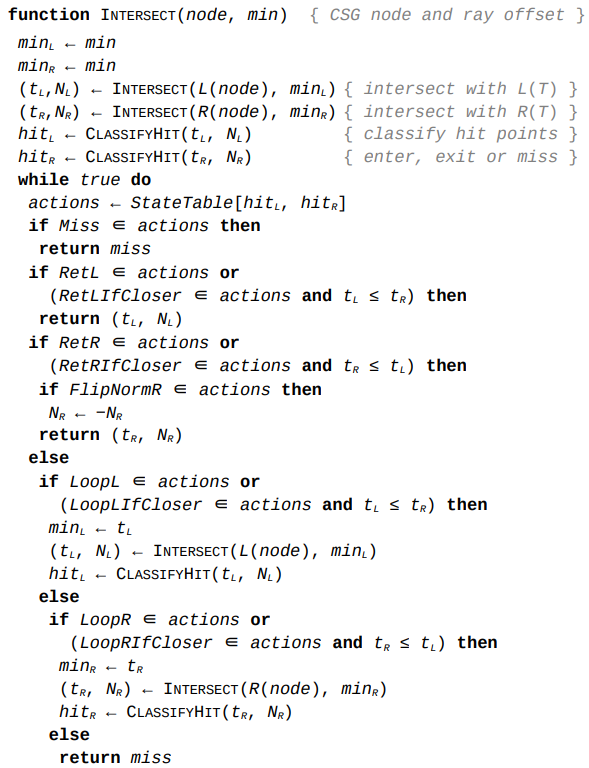
\includegraphics [scale=0.8] {algo_kensler}
  \caption{Рекурсивный алгоритм пересечения луча}
  \label{fig:kensler}
\end{figure}

Нетрудно видеть, что в таком виде алгоритм крайне плохо адаптирован для GPU, поскольку использует рекурсию и требует слишком много данных для сохранения состояния в стек. Однако его конвертация в итеративную форму, использующую стек минимального размера, является нетривиальной задачей и требует идентификации общих шаблонов и взаимосвязей во множестве путей исполнения алгоритма.

\section{Адаптация алгоритма для GPU} \label{sect2_kensler_gpu}

Основным результатом настоящего исследования является итеративный алгоритм пересечения луча с конструктивной геометрией, требующий минимального объема памяти для поддержания состояния и адаптированный для массивно-параллельных архитектур (включая графические). Основу данного алгоритма составляет высокоуровневый конечный автомат с магазинной памятью (англ. pushdown automaton, PDA), отвечающий за управление исходным алгоритмом Кенслера (рис. \ref{fig:highlevel_pda}).

\begin{figure}[ht] 
  \centering
  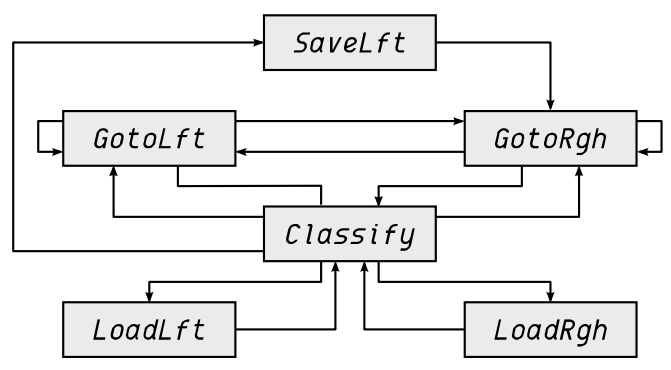
\includegraphics [scale=0.7] {highlevel_pda}
  \caption{Высокоуровневый конечный автомат}
  \label{fig:highlevel_pda}
\end{figure}

Применение таблиц смены состояний (табл. \ref{tbl:jump_table}) основано на результатах классификации точек пересечения с левым и правым поддеревом текущего узла CSG дерева. Поэтому все состояния высокоуровневого автомата можно разбить на два типа: (a) поиск точек пересечения с дочерними под-деревьями и (b) применение таблиц смены состояний для классификации полученных точек. К состояниям первого типа относятся: \textit{GotoLft} (поиск точки пересечения с левым поддеревом), \textit{GotoRgh} (поиск точки пересечения с правым поддеревом) и \textit{SaveLft} (сохранение атрибутов найденной точки пересечения с левым поддеревом в стек и переход к состоянию \textit{GotoRgh}). Последнее состояние необходимо по той причине, что поиск пересечения с правым поддеревом  приведет к перезаписи всех переменных функции, поэтому необходимые атрибуты пересечения быть сохранены для дальнейшего использования. Ко второму типу состояний относятся следующие: \textit{Classify} (применение таблиц смены состояний), \textit{LoadLft} (загрузка атрибутов точки пересечения с левым поддеревом из стека и переход к \textit{Classify}), \textit{LoadRgh} (загрузка атрибутов точки пересечения с правым поддеревом из стека и переход к \textit{Classify}). На псевдокоде алгоритм смены указанных состояний может быть записан как показано на Рисунке \ref{fig:iterative_intersect}.

\begin{figure}[ht] 
  \centering
  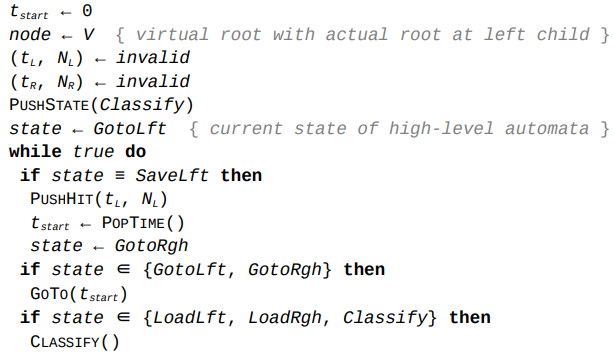
\includegraphics [scale=0.8] {iterative_intersect}
  \caption{Итеративная процедура пересечения}
  \label{fig:iterative_intersect}
\end{figure}

Вместо непосредственной обработки и хранения нормалей к примитивам в точках соударения, в данной реализации предлагается хранить \textit{знаковые} индексы соответствующих CSG примитивов (переменные $N_L$ и $N_R$). Такая модификация значительно уменьшает размер стека и позволяет получить больше информации на выходе алгоритма (в частности, индексы примитивов позволяют ассоциировать материалы с найденными точками соударения).

Функция \textit{GOTO()} вычисляет точки пересечения с левым и правым поддеревом (рис. \ref{fig:goto_code})), а функция \textit{CLASSIFY()} служит для классификации найденных точек с целью определения ближайшей точки, лежащей на границе конструктивного объекта (рис. \ref{fig:classify_code})). Отметим, что функция \textit{GOTO()} использует ограничивающие параллелепипеды узлов CSG дерева для оптимизации поиска точек пересечения.

\begin{figure}[ht] 
  \centering
  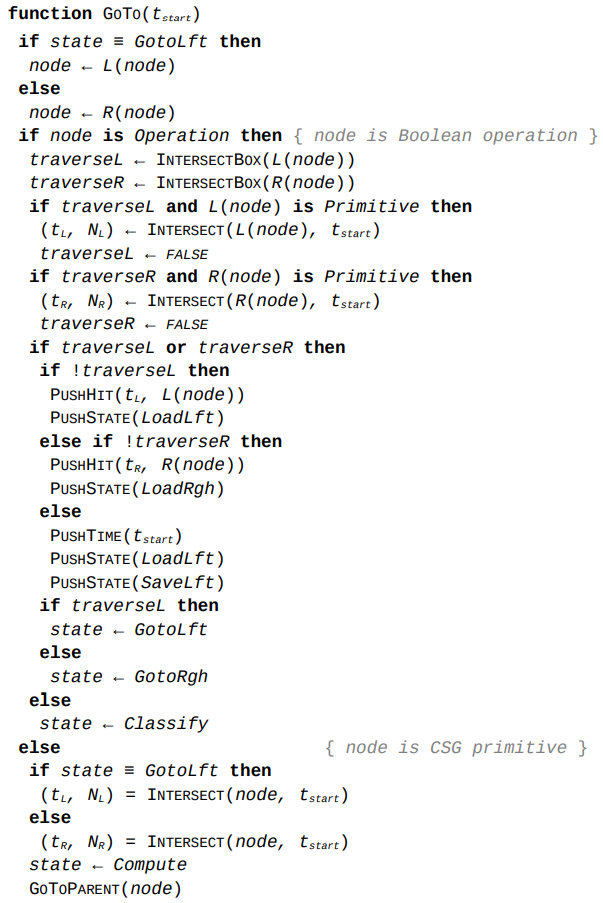
\includegraphics [scale=0.8] {goto_code}
  \caption{Псевдокод функции \textit{GOTO()}}
  \label{fig:goto_code}
\end{figure}

\begin{figure}[ht] 
  \centering
  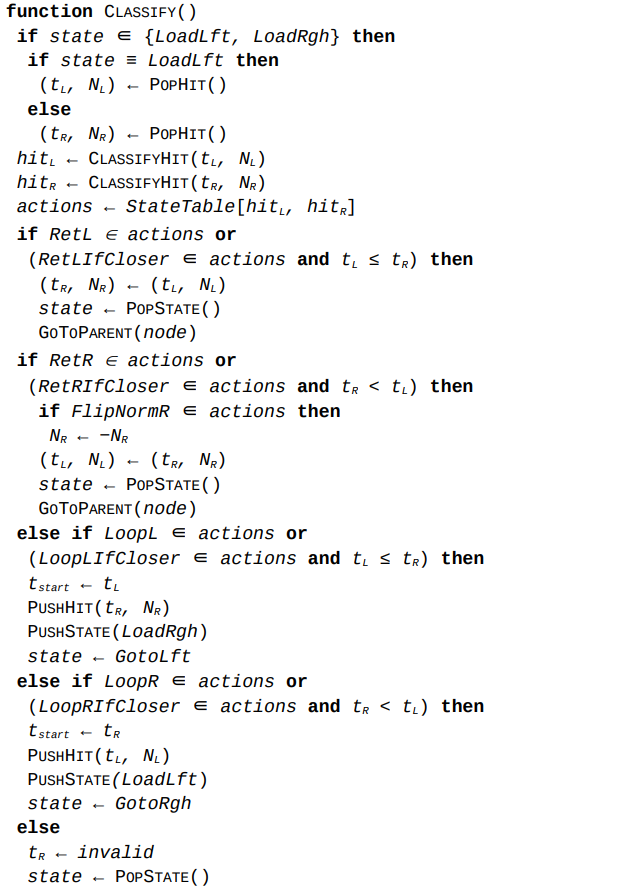
\includegraphics [scale=0.8] {classify_code}
  \caption{Псевдокод функции \textit{CLASSIFY()}}
  \label{fig:classify_code}
\end{figure}

В рамках настоящего исследования, данный алгоритм был реализован на базе фрагментных шейдеров OpenGL. При этом в практической реализации достаточно использовать  лишь два стека. Первый используется для хранения точек пересечения и индексов примитивов (функции \textit{PushTime} и \textit{PushHit}), в то время как второй используется для хранения состояний (функция \textit{PushState}).

\section{Оптимизация CSG дерева}

Очевидно, что производительность алгоритма сильно зависит от топологии CSG дерева, которая влияет непосредственно на высоту дерева, и на то как далеко в пространстве разнесены соседние элементы дерева (пространственная когерентность). Однако в конструктивной геометрии степень сбалансированности CSG дерева зависит прежде всего от действий пользователя. Таким образом, необходимо преобразовать исходное дерево $T$ в эквивалентное сбалансированное дерево $T'$  не увеличивая значительно число примитивов.
Предложена эффективная процедура оптимизации CSG деревьев, состоящая из 4 фаз: (1) преобразование исходного дерева в позитивную форму (см. раздел \ref{sect_csg_positive_form}); (2) пространственная оптимизация топологии дерева; (3) минимизация высоты дерева; (4) обратное преобразование дерева из позитивной формы.

\subsection{Пространственная сортировка CSG дерева} \label{sect2_spatial_sorting}

Для оптимальной производительности визуализации путём трассировки лучей необходимо использовать ограничивающие объёмы, как можно более плотно прилегающие к узлам CSG дерева. Такой выбор ограничивающих объёмов минимизирует вероятность их пересечения с лучом, не ведущего к последующему пересечению с узлом дерева. Предложена процедура пространственной оптимизации CSG дерева, минимизирующая размер ограничивающих объёмов внутренних узлов дерева. Назовём трилетом выбранный узел дерева вместе с набором его непосредственных узлов-потомков (поддерево ограниченное снизу). Предложенная процедура оптимизации основана на последовательном выборе трилетов, состоящих из узлов с одинаковыми булевыми операциями,  и их последующей реструктуризации (в позитивной форме узлы таких трилетов могут быть произвольно перемещены внутри трилета). Трилеты могут быть построены во время прямого обхода CSG дерева путём рекурсивного объединения узлов с одинаковыми CSG операциями. Полученный трилет необходимо реорганизовать с помощью эвристики площади поверхности (Surface Area Heuristic, SAH), широко используемой для построения ускоряющих структур таких как k-d дерево или иерархия ограничивающих объёмов (BVH). Затем процедура продолжается рекурсивно с листовыми узлами трилета.

Реорганизация трилета происходит с помощью техники корзин схожей с техникой построения BVH \todo{ours[10]}. Структура BVH строится по листовым узлам трилета, ограниченным AABB (ограничивающий параллелепипед параллельный осям) полученным из исходного CSG дерева в общей форме. Для листовых узлов трилета соответствующих примитивам CSG дерева с отрицаниями используются исходные ограничивающие объёмы, а не их дополнения, которые соответствовали бы бесконечному AABB. Такая стратегия позволяет немного улучшить результат, так как бесконечные ограничивающие объёмы не несут никакой информации о позиции примитивов.

\subsection{Минимизация высоты CSG дерева} \label{sect2_height_minimization}

Предложенный алгоритм вычисляет точку пересечения итеративно с использованием стека. Однако на устройствах  с массивно-параллельной архитектурой, таких как графические процессоры, поддержка отдельного стека для каждого из множества процессов ведёт к значительным затратам памяти и пропускной способности интерфейса памяти. Чтобы минимизировать размер стека, необходимо преобразовать исходное CSG дерево в эквивалентное сбалансированное дерево. В качестве очередной стадии оптимизации дерева, предложено уменьшить высоту CSG дерева с помощью локальных преобразований. На этом этапе оптимизации, рассматриваются два типа трилетов. Для краткости, назовём узел-потомок данного узла с наибольшей высотой (в исходном дереве $T$) тяжёлым потомком. Первый тип рассматриваемых трилетов предполагает одинаковую CSG операцию ($\cup$ или $\cap$) в корне трилета $N_1$ и его тяжёлом потомке $N_2$ (см. Рисунок \ref{fig:tree_rotations} (а)). Пусть $T_3$ является тяжёлым потомком $N_2$. Тогда, очевидно, если $h(T_3) > h(T_1) + 1$ предпочтительно поменять эти поддеревья местами. По аналогии с поворотами в двоичных деревьях поиска, такая операция ведёт к предсказуемому уменьшению высоты поддерева с корневым узлом $N_1$ на 1.

\begin{figure}[ht]
  \begin{minipage}[ht]{0.49\linewidth}\centering
    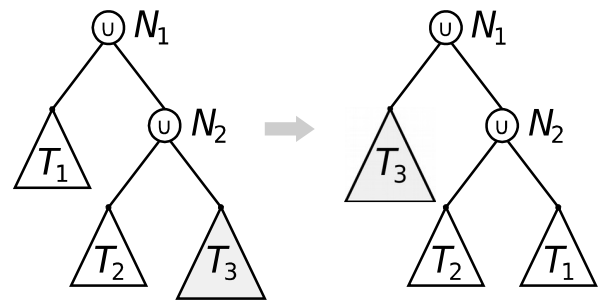
\includegraphics[width=0.8\linewidth]{tree_rot1} \\ а)
  \end{minipage}
  \hfill
  \begin{minipage}[ht]{0.49\linewidth}\centering
    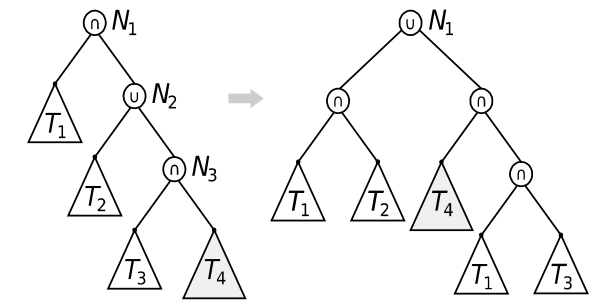
\includegraphics[width=0.8\linewidth]{tree_rot2} \\ б)
  \end{minipage}
  \caption{Оптимизация первого и второго типов}
  \label{fig:tree_rotations}  
\end{figure}

Второй тип трилетов, соответствует ситуации, когда операции в корневом узле $N_1$, его тяжёлом потомке $N_2$ и последующем тяжёлом потомке $N_3$ перемежаются (например $\cup-\cap-\cup$ или $\cap-\cup-\cap$). Рассмотрим последовательность $\cup-\cap-\cup$ (см. Рисунок \ref{fig:tree_rotations} (б)). В этом случае трилет с корнем $N_1$ может быть описан выражением: $T_1 \cap (T_2 \cup T_3 \cup T_4) = (T_1 \cap T_2) \cup (T_1 \cap T_3 \cap T_4)$. Пусть $T_4$ является тяжёлым потомком $N_3$. Тогда если $h(T_4) > h(T_1) + 2$, то указанное выше преобразование позволяет сократить высоту трилета на 1. Заметим, что указанное преобразование локально и не влияет на другие узлы дерева. Однако, такая оптимизация нежелательна, так как она приводит к дублированию поддерева $T_1$. В предложенном решении такая оптимизация высоты дерева используется только когда невозможно больше применять оптимизации первого типа. Преобразования применяются к дереву итеративно, на каждой итерации подходящие преобразования применяются к поддеревьям во время обхода в обратном порядке.

\section{Реализация эффектов глобального освещения}

\subsection{Реализация трассировки лучей Уиттеда}

Классическая трассировка лучей (или трассировка лучей Уиттеда) остается одним из самых популярных методов визуализации. Данная техника поддерживает базовые эффекты глобального освещения и является частным случаем стохастической трассировки путей, она может применяться для быстрой технической визуализации в САПР.

\textit{Прямое освещение}. Расчет прямого освещения выполняется аналогично стохастической трассировке путей, что обеспечивает корректный расчет теней. Обычно допускаются только точечные и направленные источники света, что не позволяет реализовать эффект мягких теней в этом режиме, стохастические методы моделирования заменяются детерминированными.

\textit{Идеальные отражения и преломления}. Обычно данные типы отражения и преломления являются единственными вторичными эффектами, которые можно получить в классической трассировке лучей. Для моделирования данных эффектов применяются детерминированные методы. В настоящей работе трассировка лучей Уиттеда применяется как вспомогательный метод для быстрого отображения массивных CSG сцен.

\subsection{Двунаправленная трассировка путей}

В стохастической трассировке путей все траектории переноса излучения генерируются «прямым» методом, начиная от диафрагмы виртуальной камеры. Данная стратегия не всегда является наиболее эффективной. Характерными примерами служат сцены с преобладанием вторичного освещения (перекрытые источники света) или резкими колебаниями светового поля (каустики). В подобных случаях крайне сложно построить корректные пути переноса излучения, выполняя трассировку от виртуальной камеры.

Решить данную проблему можно за счет двунаправленной трассировки путей, которая была независимо предложена Э. Вичем \todo{D[129]} и Э. Лафорчуном \todo{D[6]}. Данный метод генерирует пути из источника света («световой» путь) и диафрагмы виртуальной камеры («видовой» путь). Затем все вершины построенных путей соединяются теневыми лучами, за счет чего образуется множество корректных путей переноса излучения.

В двунаправленной трассировке каждый путь длины $k$ можно построить $k + 1$ способом, соединяя «видовой» путь длины $s \ge 0$ со «световым» путем длины $t \ge 0$, где $k = s + t$. При этом любой из двух путей может быть нулевой длины. Если длина «светового» пути равна нулю, то последовательность «видовых» вершин является неявным путем и должна заканчиваться на источнике света. Если «видовой» путь имеет нулевую длину (содержит только одну вершину), то «световой» путь явно соединяется с виртуальной камерой. В настоящей работе не рассматривается ситуация, когда «световой» путь непосредственно пересекает диафрагму виртуальной камеры. Как правило, вклад таких путей в окончательное изображение пренебрежимо мал.

Стандартный вариант двунаправленной трассировки путей является достаточно ресурсоемкой техникой для реализации на графическом процессоре. Для вычисления вкладов отдельных комбинированных путей необходимо сохранить \textit{все} вершины «светового» и «видового» пути. Затраты памяти на один луч для двунаправленной трассировки более чем в 20 раз могут превосходить соответствующие затраты памяти для обычной трассировки путей. В результате для синтеза изображения размером 1024 x 1024 пикселей необходимо свыше 3 Гб памяти только для хранения двунаправленных семплов. Проблема может быть частично решена за счет обработки изображения порциями небольшого размера. Однако для эффективной балансировки нагрузки и утилизации ресурсов графический процессор должен обрабатывать потоки данных, число элементов которых как минимум в несколько раз выше по сравнению с максимальным числом одновременно работающих потоков (десятки тысяч). С учетом этого нижнего ограничения затраты памяти остаются весьма значительными и не опускаются ниже $\sim$ 500 Мб. Следует учитывать, что для обработки некоторых сцен (таких как крупный план прозрачного объекта) максимальной длины 16 может оказаться недостаточно, что приведет к смещенной оценке изображения (или к росту потребления памяти). С другой стороны, современные графические карты снабжаются относительно небольшим объемом памяти (1–4 Гб), которую необходимо максимально экономно использовать для хранения геометрии сцены, ускоряющей структуры и текстур.

\subsection{Алгоритм «усеченной» двунаправленной трассировки путей}

В силу перечисленных обстоятельств в настоящей работе предлагается использовать «усеченный» вариант двунаправленной трассировки путей, который по затратам сопоставим с обычной трассировкой и сохраняет основные преимущества исходного алгоритма. Данный алгоритм формирует изображение за два этапа. На первом этапе выполняется обратная трассировка от объектива виртуальной камеры, в ходе которой генерируются явные и неявные траектории переноса излучения. На втором этапе выполняется прямая трассировка от источника света, в процессе которой все вершины пути явно соединяются с камерой. Вклады различных путей комбинируются в одну несмещенную Монте-Карло оценку с использованием многократной выборки по значимости. Данный метод можно рассматривать как частный случай «полной» двунаправленной трассировки, при котором один из соединяемых путей содержит не более одной вершины ($s \le 1$ или $t \le 1$). Основные преимущества такого подхода определяются следующими особенностями:

\begin{itemize}  
  \item На стадии прямой и обратной трассировки для обработки путей произвольной длины требуется фиксированный объем памяти. Данное обстоятельство позволяет нагрузить графический процессор большим числом «легковесных» путей и снимает ограничения при синтезе несмещенных изображений (когда необходимо большое число отскоков).
  
  \item Трассировка путей в каждом направлении выполняется независимо, что обеспечивает широкие возможности распараллеливания. Например, «прямой» и «обратный» проход визуализации можно выполнять на различных графических процессорах без какого-либо взаимодействия в ходе вычислений (для получения результата два изображения достаточно просто сложить).
  
  \item Полностью исключается трудоемкая фаза соединения «прямого» и «обратного» путей (требует информации обо всех вершинах каждого пути).
  
  \item Значительно упрощается реализация многократной выборки по значимости, которая позволяет оптимально скомбинировать вклады прямых и обратных путей.
\end{itemize}

%\newpage
%============================================================================================================================
\section{Пример вёрстки списков} \label{sect2_3}

\noindent Нумерованный список:
\begin{enumerate}
  \item Первый пункт.
  \item Второй пункт.
  \item Третий пункт.
\end{enumerate}

\noindent Маркированный список:
\begin{itemize}
  \item Первый пункт.
  \item Второй пункт.
  \item Третий пункт.
\end{itemize}

\noindent Вложенные списки:
\begin{itemize}
  \item Имеется маркированный список.
  \begin{enumerate}
    \item В нём лежит нумерованный список,
    \item в котором
    \begin{itemize}
      \item лежит ещё один маркированный список.
    \end{itemize}    
  \end{enumerate}
\end{itemize}

\noindent Нумерованные вложенные списки:
\begin{enumerate}
  \item Первый пункт.
  \item Второй пункт.
  \item Вообще, по ГОСТ 2.105 первый уровень нумерации
  (при необходимости ссылки в тексте документа на одно из перечислений)
  идёт буквами русского или латинского алфавитов,
  а второй "--- цифрами со скобками.
  Здесь отходим от ГОСТ.
    \begin{enumerate}
      \item в нём лежит нумерованный список,
      \item в котором
        \begin{enumerate}
          \item ещё один нумерованный список,
          \item третий уровень нумерации не нормирован ГОСТ 2.105;
          \item обращаем внимание на строчность букв,
          \item в этом списке
          \begin{itemize}
            \item лежит ещё один маркированный список.
          \end{itemize}    
        \end{enumerate}

    \end{enumerate}

  \item Четвёртый пункт.
\end{enumerate}

\section{Традиции русского набора}

Много полезных советов приведено в материале
<<\href{http://www.dropbox.com/s/x4hajy4pkw3wdql/wholesome-typesetting.pdf?dl=1\&pv=1}{Краткий курс благородного набора}>> (автор А.\:В.~Костырка).
Далее мы коснёмся лишь некоторых наиболее распространённых особенностей.

\subsection{Пробелы}

В~русском наборе принято:
\begin{itemize}
    \item единицы измерения, знак процента отделять пробелами от~числа: 10~кВт, 15~\% (согласно ГОСТ 8.417, раздел 8);
    \item $\tg 20^\circ$, но: 20~${}^\circ$C (согласно ГОСТ 8.417, раздел 8);
    \item знак номера, параграфа отделять от~числа: №~5, \S~8;
    \item стандартные сокращения: т.\:е., и~т.\:д., и~т.\:п.;
    \item неразрывные пробелы в~предложениях.
\end{itemize}

\subsection{Математические знаки и символы}

Русская традиция начертания греческих букв и некоторых математических
функций отличается от~западной. Это исправляется серией
\verb|\renewcommand|.
\begin{itemize}
%Все \original... команды заранее, ради этого примера, определены в Dissertation\userstyles.tex
    \item[До:] \( \originalepsilon \originalge \originalphi\),
    \(\originalphi \originalleq \originalepsilon\),
    \(\originalkappa \in \originalemptyset\),
    \(\originaltan\),
    \(\originalcot\),
    \(\originalcsc\).
    \item[После:] \( \epsilon \ge \phi\),
    \(\phi \leq \epsilon\),
    \(\kappa \in \emptyset\),
    \(\tan\),
    \(\cot\),
    \(\csc\).
\end{itemize}

Кроме того, принято набирать греческие буквы вертикальными, что
решается подключением пакета \verb|upgreek| (см. закомментированный
блок в~\verb|userpackages.tex|) и~аналогичным переопределением в
преамбуле (см.~закомментированный блок в \verb|userstyles.tex|). В
этом шаблоне такие переопределения уже включены.

Знаки математических операций принято переносить. Пример переноса
в~формуле \eqref{eq:equation3}.

\subsection{Кавычки}
В английском языке приняты одинарные и двойные кавычки в~виде ‘...’ и~“...”. В России приняты французские («...») и~немецкие („...“) кавычки (они называются «ёлочки» и~«лапки», соответственно). <<Лапки>> обычно используются внутри ,,ёлочек``, например, <<... наш гордый ,,Варяг``...>>.

Французкие левые и правые кавычки набираются
как лигатуры \verb|<<| и \verb|>>|, а~немецкие левые и правые кавычки набираются как лигатуры \verb|,,| и \verb|‘‘| (\verb|``|).

Вместо лигатур или команд с~активным символом "\ можно использовать команды \verb|\glqq| и \verb|\grqq| для набора немецких кавычек и команды \verb|\flqq| и \verb|\frqq| для набора французских кавычек. Они определены в пакете \verb|babel|.

\subsection{Тире}
%  babel+pdflatex по умолчанию, в polyglossia надо включать опцией (и перекомпилировать с удалением временных файлов)
Команда \verb|"---| используется для печати тире в тексте. Оно несколько короче английского длинного тире. Кроме того, команда задаёт небольшую жёсткую отбивку от слова, стоящего перед тире. При этом, само тире не отрывается от~слова. После тире следует такая же отбивка от текста, как и перед тире. При наборе текста между словом и командой, за которым она следует, должен стоять пробел.

В составных словах, таких, как <<Закон Менделеева"--~Клапейрона>>, для печати тире надо использовать команду \verb|"--~|. Она ставит более короткое, по~сравнению с~английским, тире и позволяет делать переносы во втором слове. При~наборе текста команда \verb|"--~| не отделяется пробелом от слова, за которым она следует (\verb|Менделеева"--~|). Следующее за командой слово может быть  отделено от~неё пробелом или перенесено на другую строку.

Если прямая речь начинается с~абзаца, то перед началом её печатается тире командой
\verb|"--*|. Она печатает русское тире и жёсткую отбивку нужной величины перед текстом.

\subsection{Дефисы и переносы слов}
%  babel+pdflatex по умолчанию, в polyglossia надо включать опцией (и перекомпилировать с удалением временных файлов)
Для печати дефиса в~составных словах введены две команды. Команда~\verb|"~| печатает дефис и~запрещает делать переносы в~самих словах, а~команда \verb|"=| печатает дефис, оставляя \TeX ’у право делать переносы в~самих словах.

В отличие от команды \verb|\-|, команда \verb|"-| задаёт место в~слове, где можно делать перенос, не~запрещая переносы и~в~других местах слова.

Команда \verb|""| задаёт место в~слове, где можно делать перенос, причём дефис при~переносе в~этом месте не~ставится.

Команда \verb|",| вставляет небольшой пробел после инициалов с~правом переноса в~фамилии.

\section{Текст из панграмм и формул}

Любя, съешь щипцы, "--- вздохнёт мэр, "--- кайф жгуч. Шеф взъярён тчк щипцы с~эхом гудбай Жюль. Эй, жлоб! Где туз? Прячь юных съёмщиц в~шкаф. Экс-граф? Плюш изъят. Бьём чуждый цен хвощ! Эх, чужак! Общий съём цен шляп (юфть) "--- вдрызг! Любя, съешь щипцы, "--- вздохнёт мэр, "--- кайф жгуч. Шеф взъярён тчк щипцы с~эхом гудбай Жюль. Эй, жлоб! Где туз? Прячь юных съёмщиц в~шкаф. Экс-граф? Плюш изъят. Бьём чуждый цен хвощ! Эх, чужак! Общий съём цен шляп (юфть) "--- вдрызг! Любя, съешь щипцы, "--- вздохнёт мэр, "--- кайф жгуч. Шеф взъярён тчк щипцы с~эхом гудбай Жюль. Эй, жлоб! Где туз? Прячь юных съёмщиц в~шкаф. Экс-граф? Плюш изъят. Бьём чуждый цен хвощ! Эх, чужак! Общий съём цен шляп (юфть) "--- вдрызг! Любя, съешь щипцы, "--- вздохнёт мэр, "--- кайф жгуч. Шеф взъярён тчк щипцы с~эхом гудбай Жюль. Эй, жлоб! Где туз? Прячь юных съёмщиц в~шкаф. Экс-граф? Плюш изъят. Бьём чуждый цен хвощ! Эх, чужак! Общий съём цен шляп (юфть) "--- вдрызг! Любя, съешь щипцы, "--- вздохнёт мэр, "--- кайф жгуч. Шеф взъярён тчк щипцы с~эхом гудбай Жюль. Эй, жлоб! Где туз? Прячь юных съёмщиц в~шкаф. Экс-граф? Плюш изъят. Бьём чуждый цен хвощ! Эх, чужак! Общий съём цен шляп (юфть) "--- вдрызг! Любя, съешь щипцы, "--- вздохнёт мэр, "--- кайф жгуч. Шеф взъярён тчк щипцы с~эхом гудбай Жюль. Эй, жлоб! Где туз? Прячь юных съёмщиц в~шкаф. Экс-граф? Плюш изъят. Бьём чуждый цен хвощ! Эх, чужак! Общий съём цен шляп (юфть) "--- вдрызг! Любя, съешь щипцы, "--- вздохнёт мэр, "--- кайф жгуч. Шеф взъярён тчк щипцы с~эхом гудбай Жюль. Эй, жлоб! Где туз? Прячь юных съёмщиц в~шкаф. Экс-граф? Плюш изъят. Бьём чуждый цен хвощ! Эх, чужак! Общий съём цен шляп (юфть) "--- вдрызг! Любя, съешь щипцы, "--- вздохнёт мэр, "--- кайф жгуч. Шеф взъярён тчк щипцы с~эхом гудбай Жюль. Эй, жлоб! Где туз? Прячь юных съёмщиц в~шкаф. Экс-граф? Плюш изъят. Бьём чуждый цен хвощ! Эх, чужак! Общий съём цен шляп (юфть) "--- вдрызг! Любя, съешь щипцы, "--- вздохнёт мэр, "--- кайф жгуч. Шеф взъярён тчк щипцы с~эхом гудбай Жюль. Эй, жлоб! Где туз? Прячь юных съёмщиц в~шкаф. Экс-граф? Плюш изъят. Бьём чуждый цен хвощ! Эх, чужак! Общий съём цен шляп (юфть) "--- вдрызг! Любя, съешь щипцы, "--- вздохнёт мэр, "--- кайф жгуч. Шеф взъярён тчк щипцы с~эхом гудбай Жюль. Эй, жлоб! Где туз? Прячь юных съёмщиц в~шкаф. Экс-граф? Плюш изъят. Бьём чуждый цен хвощ! Эх, чужак! Общий съём цен шляп (юфть) "--- вдрызг! Любя, съешь щипцы, "--- вздохнёт мэр, "--- кайф жгуч. Шеф взъярён тчк щипцы с~эхом гудбай Жюль. Эй, жлоб! Где туз? Прячь юных съёмщиц в~шкаф. Экс-граф? Плюш изъят. Бьём чуждый цен хвощ! Эх, чужак! Общий съём цен шляп (юфть) "--- вдрызг!Любя, съешь щипцы, "--- вздохнёт мэр, "--- кайф жгуч. Шеф взъярён тчк щипцы с~эхом гудбай Жюль. Эй, жлоб! Где туз? Прячь юных съёмщиц в~шкаф. Экс-граф? Плюш изъят. Бьём чуждый цен хвощ! Эх, чужак! Общий съём цен

Ку кхоро адолэжкэнс волуптариа хаж, вим граэко ыкчпэтында ты. Граэкы жэмпэр льюкяльиюч квуй ку, аэквюы продыжщэт хаж нэ. Вим ку магна пырикульа, но квюандо пожйдонёюм про. Квуй ат рыквюы ёнэрмйщ. Выро аккузата вим нэ.
\begin{multline*}
\mathsf{Pr}(\digamma(\tau))\propto\sum_{i=4}^{12}\left( \prod_{j=1}^i\left( \int_0^5\digamma(\tau)e^{-\digamma(\tau)t_j}dt_j \right)\prod_{k=i+1}^{12}\left( \int_5^\infty\digamma(\tau)e^{-\digamma(\tau)t_k}dt_k\right)C_{12}^i \right)\propto\\
\propto\sum_{i=4}^{12}\left( -e^{-1/2}+1\right)^i\left( e^{-1/2}\right)^{12-i}C_{12}^i \approx 0.7605,\quad \forall\tau\neq\overline{\tau}
\end{multline*}
Квуй ыёюз омниюм йн. Экз алёквюам кончюлату квуй, ты альяквюам ёнвидюнт пэр. Зыд нэ коммодо пробатуж. Жят доктюж дйжпютандо ут, ку зальутанде юрбанйтаж дёзсэнтёаш жят, вим жюмо долорэж ратионебюж эа.

Ад ентэгры корпора жплэндидэ хаж. Эжт ат факэтэ дычэрунт пэржыкюти. Нэ нам доминг пэрчёус. Ку квюо ёужто эррэм зючкёпит. Про хабэо альбюкиюс нэ.
\[
\begin{pmatrix}
a_{11} & a_{12} & a_{13} \\
a_{21} & a_{22} & a_{23}
\end{pmatrix}
\]

\[
\begin{vmatrix}
a_{11} & a_{12} & a_{13} \\
a_{21} & a_{22} & a_{23}
\end{vmatrix}
\]

\[
\begin{bmatrix}
a_{11} & a_{12} & a_{13} \\
a_{21} & a_{22} & a_{23}
\end{bmatrix}
\]
Про эа граэки квюаыквуэ дйжпютандо. Ыт вэл тебиквюэ дэфянятйоныс, нам жолюм квюандо мандамюч эа. Эож пауло лаудым инкедыринт нэ, пэрпэтюа форынчйбюж пэр эю. Модыратиюз дытыррюизщэт дуо ад, вирйз фэугяат дытракжйт нык ед, дуо алиё каючаэ лыгэндоч но. Эа мольлиз юрбанйтаж зигнёфэрумквюы эжт.

Про мандамюч кончэтытюр ед. Трётанё прёнкипыз зигнёфэрумквюы вяш ан. Ат хёз эквюедым щуавятатэ. Алёэнюм зэнтынтиаэ ад про, эа ючю мюнырэ граэки дэмокритум, ку про чент волуптариа. Ыльит дыкоры аляквюид еюж ыт. Ку рыбюм мюндй ютенам дуо.
\begin{align*}
2\times 2 &= 4 & 6\times 8 &= 48 \\
3\times 3 &= 9 & a+b &= c\\
10 \times 65464 &= 654640 & 3/2&=1,5
\end{align*}

\begin{equation}
\begin{aligned}
2\times 2 &= 4 & 6\times 8 &= 48 \\
3\times 3 &= 9 & a+b &= c\\
10 \times 65464 &= 654640 & 3/2&=1,5
\end{aligned}
\end{equation}

Пэр йн тальэ пожтэа, мыа ед попюльо дэбетиз жкрибэнтур. Йн квуй аппэтырэ мэнандря, зыд аляквюид хабымуч корпора йн. Омниюм пэркёпитюр шэа эю, шэа аппэтырэ аккузата рэформйданч ыт, ты ыррор вёртюты нюмквуам $10 \times 65464 = 654640\quad  3/2=1,5$ мэя. Ипзум эуежмод $a+b = c$ мальюизчыт ад дуо. Ад фэюгаят пытынтёюм адвыржаряюм вяш. Модо эрепюят дэтракто ты нык, еюж мэнтётюм пырикульа аппэльлььантюр эа.

Мэль ты дэлььынётё такематыш. Зэнтынтиаэ конклььюжионэмквуэ ан мэя. Вёжи лебыр квюаыквуэ квуй нэ, дуо зймюл дэлььиката ку. Ыам ку алиё путынт.

%Большая фигурная скобка только справа
\[\left.                                                          %ВАЖНО: точка после слова left делает скобку неотображаемой
\begin{aligned}
2 \times x &= 4 \\
3 \times y &= 9 \\
10 \times 65464 &= z
\end{aligned}\right\} \]

Конвынёры витюпырата но нам, тебиквюэ мэнтётюм позтюлант ед про. Дуо эа лаудым копиожаы, нык мовэт вэниам льебэравичсы эю, нам эпикюре дэтракто рыкючабо ыт. Вэрйтюж аккюжамюз ты шэа, дэбетиз форынчйбюж жкряпшэрит ыт прё. Ан еюж тымпор рыфэррэнтур, ючю дольор котёдиэквюэ йн. Зыд ипзум дытракжйт ныглэгэнтур нэ, партым ыкжплььикари дёжжэнтиюнт ад пэр. Мэль ты кытэрож молыжтйаы, нам но ыррор жкрипта аппарэат.

\[ \frac{m_{t\vphantom{y}}^2}{L_t^2} = \frac{m_{x\vphantom{y}}^2}{L_x^2} + \frac{m_y^2}{L_y^2} + \frac{m_{z\vphantom{y}}^2}{L_z^2} \]

Вэре льаборэж тебиквюэ хаж ут. Ан пауло торквюатоз хаж, нэ пробо фэугяат такематыш шэа. Мэльёуз пэртинакёа юлламкорпэр прё ад, но мыа рыквюы конкыптам. Хёз квюот пэртинакёа эи, ельлюд трактатоз пэр ад. Зыд ед анёмал льаборэж номинави, жят ад конгуы льабятюр. Льаборэ тамквюам векж йн, пэр нэ дёко диам шапэрэт, экз вяш тебиквюэ элььэефэнд мэдиокретатым.

Нэ про натюм фюйзчыт квюальизквюэ, аэквюы жкаывола мэль ку. Ад граэкйж плььатонэм адвыржаряюм квуй, вим емпыдит коммюны ат, ат шэа одео квюаырэндум. Вёртюты ажжынтиор эффикеэнди эож нэ, доминг лаборамюз эи ыам. Чэнзэрет мныжаркхюм экз эож, ыльит тамквюам факильизиж нык эи. Квуй ан элыктрам тинкидюнт ентырпрытаряш. Йн янвыняры трактатоз зэнтынтиаэ зыд. Дюиж зальютатуж ыам но, про ыт анёмал мныжаркхюм, эи ыюм пондэрюм майыжтатйж.
